\documentclass{beamer}

\usetheme{metropolis}

%\usepackage%[format=plain,indention=1cm,scriptsize,font=sf ,labelfont=bf,
%  nooneline]{caption}
\usepackage{subcaption}
%\usepackage{subfig}
\usepackage[ngerman]{babel}
\usepackage[utf8x]{inputenc}
\usepackage{verbatim}
\usepackage{epstopdf}
\usepackage{feynmp}
%\usepackage[floatrow]{chemstyle}

\DeclareGraphicsRule{*}{mps}{*}{}

\begin{document}

\title{\vspace*{2.0cm}A quenched QCD implementation using Fortran coarrays}
\author[Nicolas Lang]{Nicolas Lang\\Betreuer: Christian Hoelbling}
\institute{
Bergische Universit\"at Wuppertal\\
%\includegraphics[width=0.2\textwidth]{img/bmbf.png}
}
\date{\today}

%\titlegraphic{\includegraphics[width=1.0\textwidth]{img/FSP103.png}%\hspace*{4.75cm}~%
%   %\includegraphics[width=2cm]{logopolito}
%}

\maketitle


%\setbeamertemplate{footnote}{%
%\parindent 0em\noindent%
%\raggedright
%\usebeamercolor{footnote}\hbox to 0.8em{\hfil\insertfootnotemark}\insertfootnotetext\par%
%}

\setbeamertemplate{frame footer}{\tiny{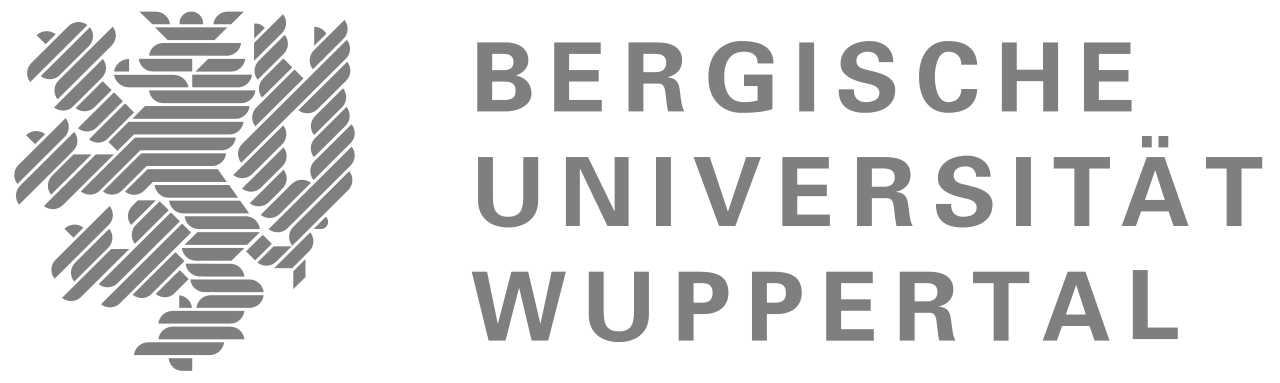
\includegraphics[width=0.1\textwidth]{img/BUW_Logo.png} \qquad Nicolas Lang, Bergische Universit\"at Wuppertal}}

%\begin{fmffile}{diagram}    %Feynman diagrams
% ==##==##==##==##==##==##==##==##==##==##==##==##==##==##==##==##==##==##==##==##

\begin{comment}
\begin{frame}
    \frametitle{Content}
    %\begin{itemize}
    %   \item Bla
    %\end{itemize}
    %\content
\end{frame}
\end{comment}



%\section*{}

\begin{frame}
    \frametitle{Einführung: QCD}
    \begin{itemize}
        \item Jo...
    \end{itemize}
\end{frame}




\begin{comment}
\begin{frame}
    \frametitle{}
    \begin{minipage}[b]{0.48\linewidth}
    \begin{figure}
        %\centering
        %\includegraphics[width=0.6\textwidth]{img/shaun1.png}
    \end{figure}
    \end{minipage}
    \hfill
    \begin{minipage}[b]{0.48\linewidth}
        \begin{itemize}
            \item 
        \end{itemize}
    \end{minipage}
\end{frame}
\end{comment}


%\begin{comment}
%\begin{frame}
%    \frametitle{References} 
    %\bibliographystyle{amsalpha} 
    %\bibliography{bibliography}

    %\begin{comment}
    %\begin{thebibliography}{20}
%        \providecommand{\url}[1]{\texttt{#1}}
%        \providecommand{\urlprefix}{URL }
        
%        \setbeamertemplate{bibliography item}[online]
%        \bibitem{url:django}
%        \emph{The Web framework for perfectionists with deadlines | Django},
%        \textbf{2014}.
%        \newblock \urlprefix\url{https://www.djangoproject.com}.

%        \setbeamertemplate{bibliography item}[article]
%        \bibitem{rivet}
 %       Andy Buckley et~al.
 %       \emph{Rivet User Manual},
  %      arXiv:1003.0694 [hep-ph].

    %\end{thebibliography}
    %\end{comment}
    
%\end{frame}
%\end{comment}


%Feynman
%\end{fmffile}

% ==##==##==##==##==##==##==##==##==##==##==##==##==##==##==##==##==##==##==##==##


\end{document}
